\documentclass[]{report}

% Define page
\usepackage[top=1in, bottom=1in, left=1.5in, right=1.5in]{geometry}
\linespread{1.1}

% For math
\usepackage{amsmath,amsthm,amssymb}
\usepackage{bm}

% For figures
\usepackage{graphicx,subfigure,psfrag}

\usepackage{natbib}

% Definitions
\newcommand{\elastix}{\texttt{elastix}}
\newcommand{\transformix}{\texttt{transformix}}
\newcommand{\vx}{\bm{x}}
\newcommand{\vu}{\bm{u}}
\newcommand{\vux}{\bm{u}(\bm{x})}
\newcommand{\vmu}{\bm{\mu}}
\newcommand{\vT}{\bm{T}}
\newcommand{\vTx}{\bm{T}(\bm{x})}

%%%%%%%%%%%%%%%%%%%%%%%%%%%%%%%%%%%%%%%%%%%%%%%%%%%%%%%%%%%%%%%%%%%%%%%%%%%%%%%%%%%%%%%%%%%%

\begin{document}

\title{Manual for \elastix}
\author{Stefan Klein and Marius Staring}
%\date{}
\maketitle

\setcounter{page}{1} \pagenumbering{roman} \tableofcontents
%\newpage
%\listoffigures
%\newpage
%\listoftables
\newpage
\pagenumbering{arabic} \setcounter{page}{1}

%%%%%%%%%%%%%%%%%%%%%%%%%%%%%%%%%%%%%%%%%%%%%%%%%%%%%%%%%%%%%%%%%%%%%%%%%%%%%%%%%%%%%%%%%%%%
% main text

\chapter{Image Registration}

\section{Introduction}

Image registration is an important tool in the field of medical
imaging. In many clinical situations several images of a patient are
made in order to analyse the patient�s situation. These images are
acquired with, for example, X-ray scanners, Magnetic Resonance
Imaging (MRI) scanners, Computed Tomography (CT) scanners, and
Ultrasound scanners, which provide knowledge about the anatomy of the
subject. Combination of patient data, mono- or multi-modal, often
yields additional clinical information not apparent in the separate
images. For this purpose, the spatial relation between the images has
to be found. Image registration is the task of finding a spatial
one-to-one mapping from voxels in one image to voxels in the other
image, see Figure \ref{fig:concept}. Good reviews on the subject are
given in \citet{HillEA01,LesterEA99,MaintzEA98}.

\begin{figure}
\centering
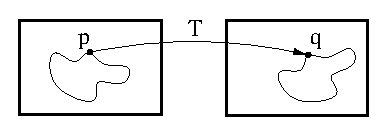
\includegraphics[width=8cm]{images/ImageRegistrationConcept.eps}
\caption{Image registration is the task of finding a spatial
transformation mapping one image to another. Adopted from
\citet{ITKSoftwareGuideSecondEdition}.} \label{fig:concept}
\end{figure}

In registration one image, what we call the \emph{moving image}
$I_M(\vx)$, is deformed to fit the other image, the \emph{fixed
image} $I_F(\vx)$. Registration is the problem of finding a
\emph{displacement} $\vux$ that makes $I_M(\vx + \vux)$ spatially
aligned to $I_F(\vx)$. An equivalent formulation is to say that
registration is the problem of finding a \emph{transformation}
$\vT(\vx) = \vx + \vux $ that makes $I_M(\vT(\vx))$ spatially aligned
to $I_F(\vx)$. The quality of alignment is defined by a distance or
similarity measure $\mathcal{S}$, such as the sum of squared
differences (SSD), the correlation ratio, or the mutual information
(MI) measure. Because this problem is ill-posed, a regularisation or
penalty term $\mathcal{P}$ is often introduced that constrains $\vT$.

Commonly, the registration problem is formulated as an optimisation
problem in which the cost function $\mathcal{C}$ is minimised w.r.t.
$\vT$:
\begin{align}
\hat \vT &= \arg \min_{\vT} \mathcal{C}(\vT; I_F,I_M), \qquad \text{with} \label{eq:registration1}\\
\mathcal{C}(\vT; I_F,I_M) &= -\mathcal{S}(\vT; I_F,I_M) + \gamma
\mathcal{P}(\vT),\label{eq:registration2}
\end{align}
where $\gamma$ weighs similarity against regularity.

\section{Images}

Since image registration is all about images, we have to be careful
with what is meant by an image. We adopt the notion of an image from
the Insight Toolkit \citep[p. 40]{ITKSoftwareGuideSecondEdition}:

\begin{quote}
Additional information about the images is considered mandatory. In
particular the information associated with the physical spacing
between pixels and the position of the image in space with respect to
some world coordinate system are extremely important. Image origin
and spacing are fundamental to many applications. Registration, for
example, is performed in physical coordinates. Improperly defined
spacing and origins will result in inconsistent results in such
processes. Medical images with no spatial information should not be
used for medical diagnosis, image analysis, feature extraction,
assisted radiation therapy or image guided surgery. In other words,
medical images lacking spatial information are not only useless but
also hazardous.

Figure \ref{fig:image} illustrates the main geometrical concepts
associated with the itk::Image. In this figure, circles are used to
represent the centre of pixels. The value of the pixel is assumed to
exist as a Dirac Delta Function located at the pixel centre. Pixel
spacing is measured between the pixel centres and can be different
along each dimension. The image origin is associated with the
coordinates of the first pixel in the image. A pixel is considered to
be the rectangular region surrounding the pixel centre holding the
data value. This can be viewed as the Voronoi region of the image
grid, as illustrated in the right side of the figure. Linear
interpolation of image values is performed inside the Delaunay region
whose corners are pixel centres.
\end{quote}

\begin{figure}
\centering
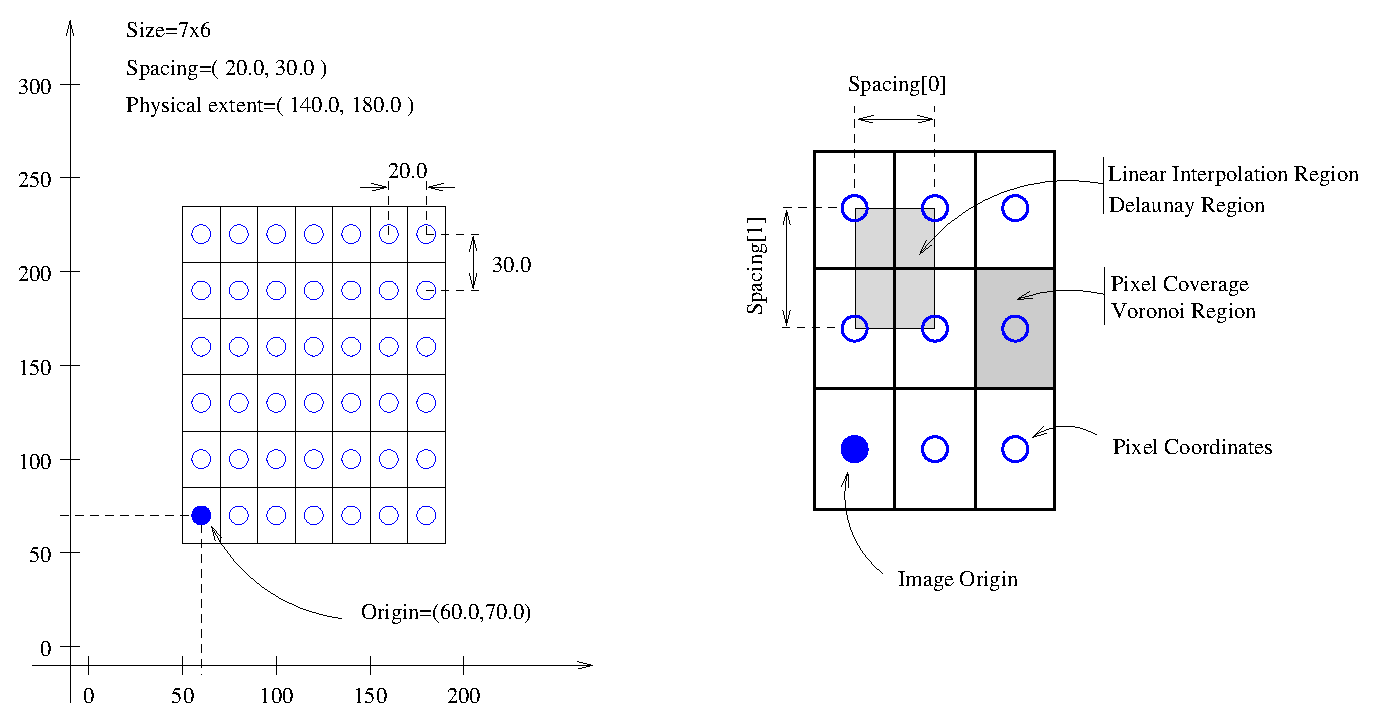
\includegraphics[width=12cm]{images/ImageOriginAndSpacing.eps}
\caption{Geometrical concepts associated with the ITK image. Adopted from
\citet{ITKSoftwareGuideSecondEdition}.} \label{fig:image}
\end{figure}

Therefore, you should take care that you use an image format that is
able to store the relevant information (e.g. mhd, DICOM).

%%%%%%%%%%%%%%%%%%%%%%%%%%%%%%%%%%%%%%%%%%%%%%%%%%%%%%%%%%%%%%%%%%%%%%%%%%%%%%%%%%%%%%%%%%%%

\chapter{Basic registration components}

From the basic registration problem formulated as in Equation
(\ref{eq:registration1}) and (\ref{eq:registration2}), several
components can be recognised. First, we have the similarity measure
$\mathcal{S}$ that defines the quality of alignment. These metrics
are discussed in Section \ref{sec:comp:metric}. Second, the
transformation model $\vT$ that defines the spatial relation, see
Section. Third, the optimisation procedure to actually solve the
problem, see Section \ref{sec:comp:optimiser}. Then, during the
optimisation the value $I_M(\vTx)$ is evaluated at non-voxel
positions, for which intensity interpolation is needed, see Section
\ref{sec:comp:interpolator}. Another thing, not immediately clear
from Equation (\ref{eq:registration1}) and (\ref{eq:registration2}),
is the use of multi-resolution strategies to speed-up registration,
and to make it more robust, see Section
\ref{sec:comp:multiresolution}. The regularisation term $\mathcal{P}$
is not discussed in this manual.

\section{Metrics}\label{sec:comp:metric}

Several choices for the similarity measure can be found in the
literature. The three most common choices are the Sum of Squared
Differences (SSD), the Normalised Correlation Coefficient (NCC), and
the Mutual Information measure (MI).

\begin{description}
\item[Sum of Squared Differences:] The SSD is defined as:
\begin{align}
\mathrm{SSD}(\vT;I_F,I_M) &= \frac{1}{N} \sum_{i=0}^N \left(
I_F(\vx_i) - I_M(\vT(\vx_i)) \right)^2,\label{eq:ssd}
\end{align}
with $N$ the number of voxels in the fixed image. Given an
transformation $\vT$, this measure can easily be implemented by
looping over the voxels in the fixed image, taking $I_F(\vx_i)$,
calculating $I_M(\vT(\vx_i))$ by interpolation, and adding the
squared difference to the sum.

\item[Normalised Correlation Coefficient:] The NCC is defined as:
\begin{align}
\mathrm{NCC}(\vT;I_F,I_M) &= \frac{ \sum_{i=0}^N \left( I_F(\vx_i) -
\overline{I_F} \right) \left( I_M(\vT(\vx_i)) - \overline{I_M}
\right) }{ \sqrt{\sum_{i=0}^N \left( I_F(\vx_i) - \overline{I_F}
\right)^2 \sum_{i=0}^N \left( I_M(\vT(\vx_i)) - \overline{I_M}
\right)^2} },\label{eq:ncc}
\end{align}
with $\overline{I_F}$ and $\overline{I_M}$ the average grey-value of
$I_F(\vx)$ and $I_M(\vT(\vx))$, respectively.

\item[Mutual Information:] For MI \citep{MaesEA97,ViolaEA97,MattesEA03} we
use a definition given by \citet{ThevenazEA00a}:
\begin{align}
\mathrm{MI}(\vT; I_F, I_M) &= \sum\limits_{\iota \in L_M}
\sum\limits_{\kappa \in L_F} p(\iota, \kappa; \vT) \log_2 \left(
\frac{ p(\iota, \kappa; \vT) }{ p_F(\kappa) p_M(\iota; \vT) }
\right),\label{eq:MI}
\end{align}
where $L_F$ and $L_M$ are the sets of histogram bin centres of the
fixed and moving image, respectively, $p$ is the joint discrete
probability, and $p_F$ and $p_M$ are the marginal discrete
probabilities. The probabilities are modelled with B-spline Parzen
windows.
\end{description}

The SSD measure is a measure that is only suited for two images with
an equal intensity distribution, i.e. for images from the same
modality. NCC is less strict, it assumes a linear relation between
the intensity values of the fixed and moving image, and can therefore
be used more often. The MI measure is the most general of the three:
only a relation between the probability distributions of the
intensities of the fixed and moving image is assumed. For the mutual
information measure it is well-known that it is suited not only for
mono-modal, but also for multi-modal image pairs. This measure is
your first choice for image registration.

\section{Transforms}\label{sec:comp:transform}

The flexibility of the transformation $\vT$ determines how much
deformation between the fixed and moving image you can handle. From
less flexibility to more we list the translation, the rigid
transformation, the affine, and finally the so-called
\emph{non-rigid} transformation. The last category covers a fast
amount of transformations, all capable to model local deformations.

\begin{description}
\item[Translation:] The translation is defined as:
\begin{align}
\vTx &= \vx + \bm{t},
\end{align}
with $\bm{t}$ a vector.

\item[Rigid:] A rigid transformation is defined as:
\begin{align}
\vTx &= R \vx + \bm{t},
\end{align}
with the matrix $R$ a rotation matrix, so it is orthonormal and
proper.

\item[Affine:] An affine transformation is defined as:
\begin{align}
\vTx &= A \vx + \bm{t},
\end{align}
where the matrix $A$ has no restrictions.

\item[B-splines:] For the category of non-rigid transformations, we focus on a
transformation that is parameterised by B-splines
\citep{RueckertEA99}. In 2D:
\begin{align}
\vT_i(\vx) &= \vx_i + \sum_{l \in V_{\vx}} \mu_{li} \beta^3(x_1 -
x_{l1}) \beta^3(x_2 - x_{l2}), \qquad \forall i \in
\{1,2\},\label{eq:bspline}
\end{align}
with $\vx = (x_1,x_2)$, $\beta^3(x)$ the cubic B-spline polynomial
\citep{Unser99}, $\mu_{li}$ the B-spline coefficients, and $V_{\vx}$
the set of all control points within the compact support of the
B-spline at $\vx$. In this context we talk about `the control point
grid that is put on the fixed image', and about `control points that
are moved around'. The control point grid is defined by the amount of
space between the control points, which can be different for each
direction. B-splines have local support, which is beneficial both for
modelling local transformations, and for fast computation. See Figure
\ref{fig:bspline} for an illustration of the use of B-splines in
image registration.
\end{description}

\begin{figure}
\centering
\subfigure[]{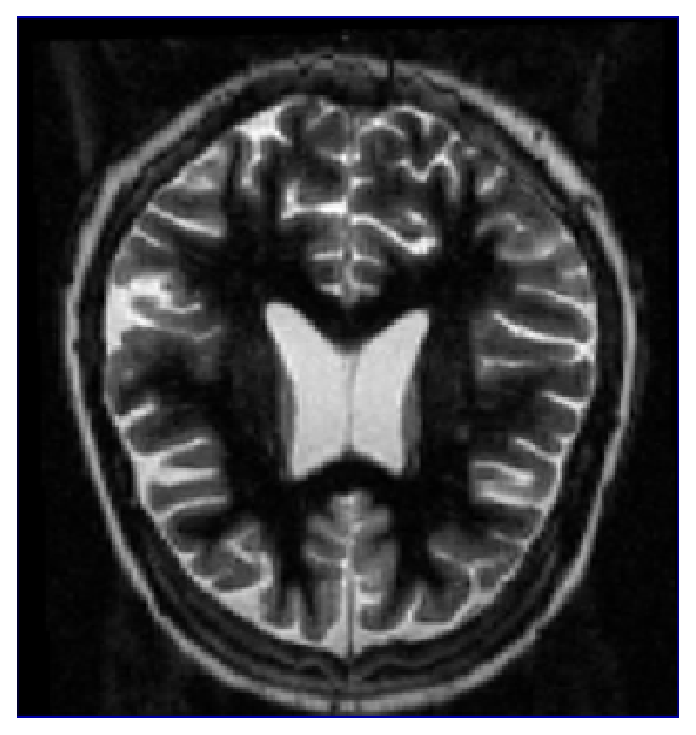
\includegraphics[width=4.5cm,height=4.5cm]{images/fixed.eps}}\label{sfig:bspline:a}
\subfigure[]{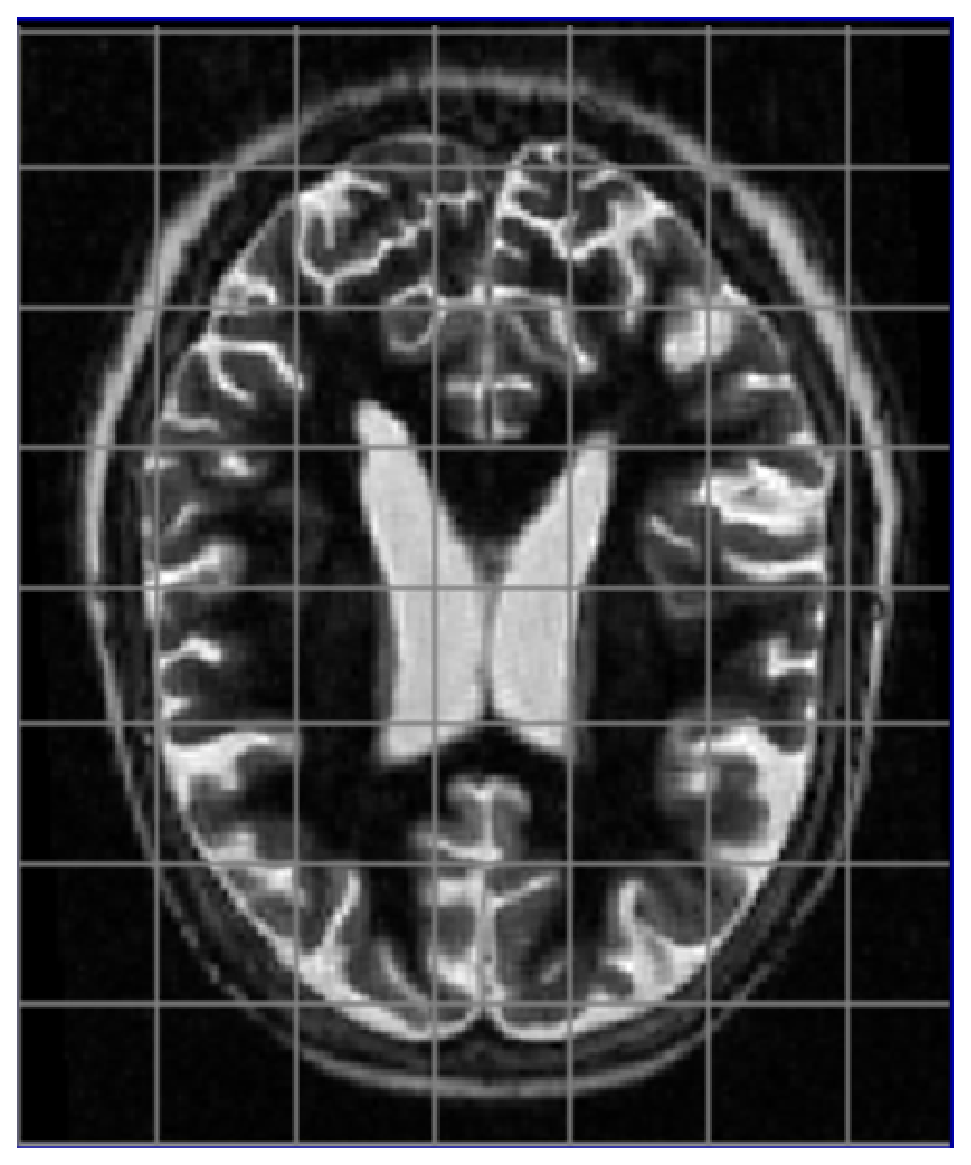
\includegraphics[width=4.5cm,height=4.5cm]{images/moving.eps}}\label{sfig:bspline:b}
\subfigure[]{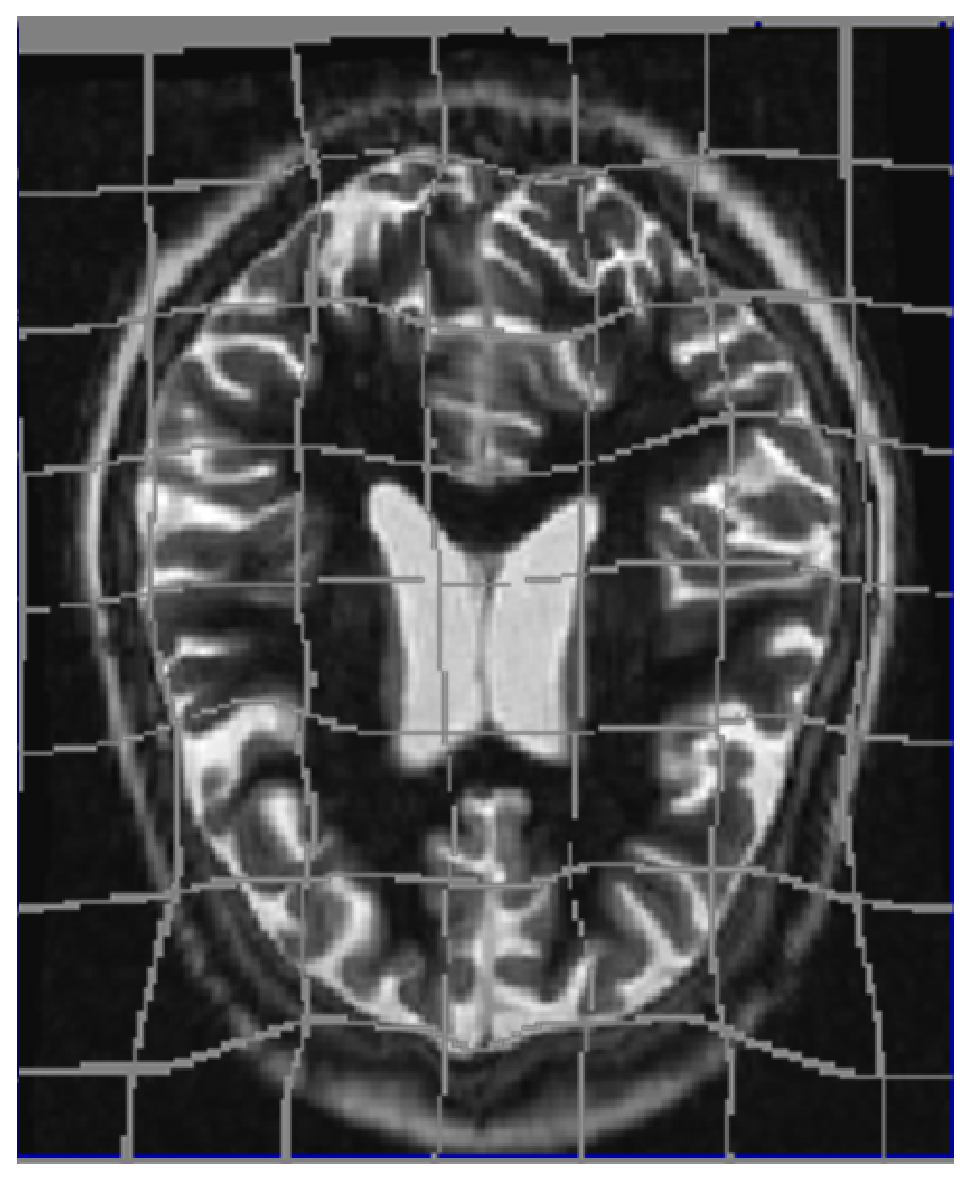
\includegraphics[width=4.5cm,height=4.5cm]{images/deformed.eps}}\label{sfig:bspline:c}
\caption{B-spline transformation. (a) the fixed image. (b) the
moving image with the B-spline grid overlayed. (c) the control points
are moved around until $I_M(\vTx)$ resembles $I_F(\vx)$. The new
deformed B-spline grid defines the deformed image.}
\label{fig:bspline}
\end{figure}

The attentive reader will notice that in Figure \ref{fig:bspline} the
B-spline grid is depicted on top of the moving image, instead of the
fixed image as stated above. This brings us to a technicality
concerning the \emph{implementation} of transformations. If a
transformation would be implemented by a so-called forward-transform,
then points from the moving image would be mapped to the fixed image
domain. However, when it comes to creating the deformed image
$I_M(\vTx)$, possibly, due to the nature of a nonrigid
transformation, none of the voxels in $I_M$ maps to a point $\bm{y}$
in the domain of $I_F$. This would result in a `gap' in the deformed
image. To avoid this, transformations are implemented using a
backward-transform. The transformation maps from the fixed image
domain to the moving image domain, and therefore the B-spline grid is
actually (`in the code') put on the fixed image.

Choose the transformation that fits your needs: only choose a
nonrigid transformation if you expect that the underlying problem
contains local deformations, choose a rigid transformation if you
only need to compensate for differences in pose. To initialise a
nonrigid registration problem, perform a rigid or affine one first.

\section{Optimisers}\label{sec:comp:optimiser}

\begin{figure}
\centering
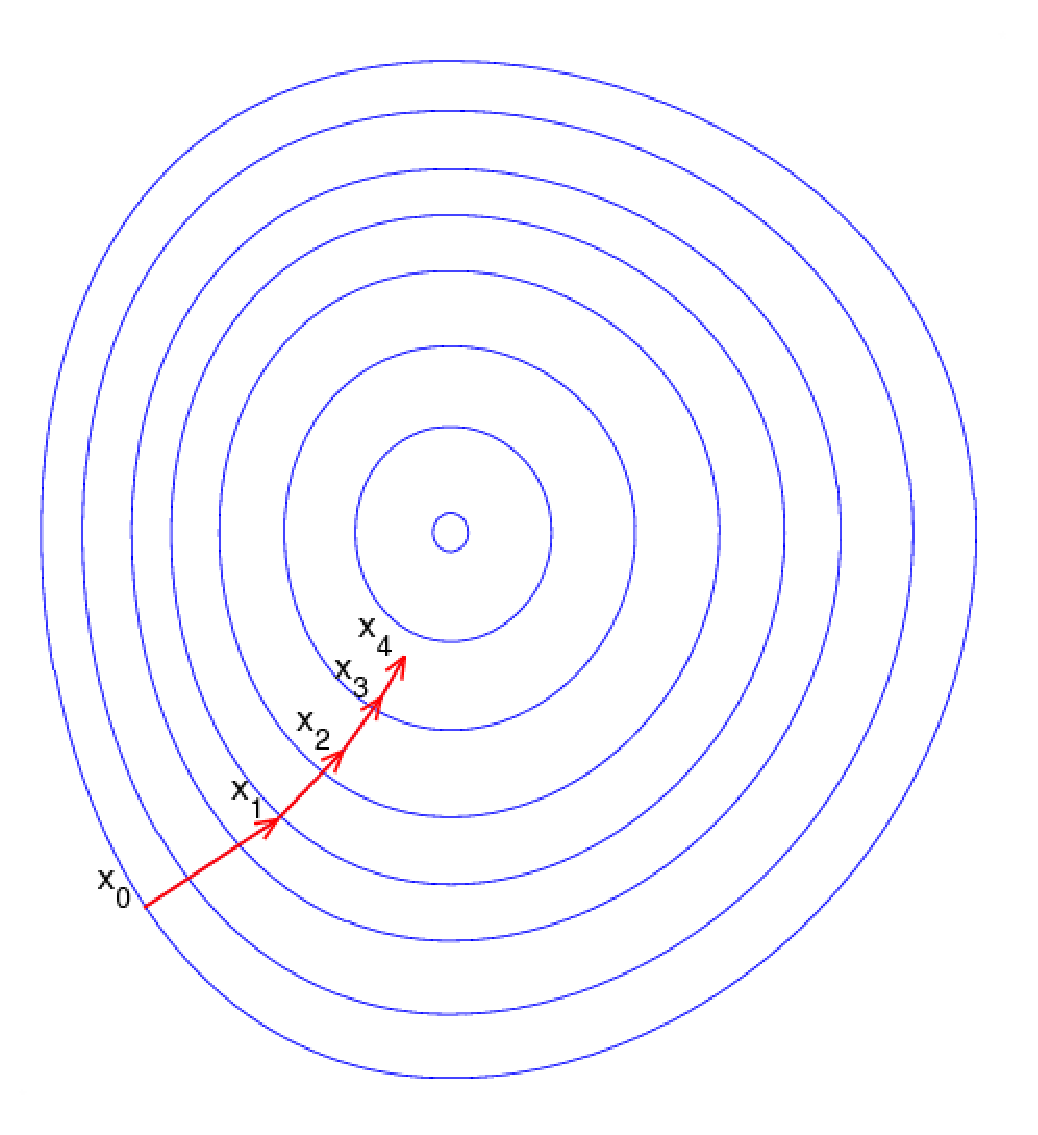
\includegraphics[width=5cm]{images/Gradient_descent.eps}
\caption{Iterative optimisation. The arrows indicate the steps
$a_k \bm{d}_k$ taken in the direction of the optimum, which is in the
centre.} \label{fig:optimisation}
\end{figure}

To solve the optimisation problem \ref{eq:registration1}, i.e. to
obtain the optimal transformation $\vT$, commonly an iterative
optimisation strategy is employed:
\begin{align}
\vmu_{k+1} &= \vmu_k + a_k \bm{d}_k, \quad k = 0, 1, 2, \cdots,
\end{align}
with $\bm{d}_k$ the `search direction' at iteration $k$, $a_k$ a
scalar gain factor controlling the step size along the search
direction, and $\vmu_k$ the parameters that define the
transformation. For example, for rigid registration the parameter
vector $\vmu$ is of size 6 in 3D: the three Euler angles and the
three translations, and for B-splines this parameters vector contains
the set of B-spline coefficients ($\mu$ in Equation
(\ref{eq:bspline}). The optimisation process is illustrated in Figure
\ref{fig:optimisation}. \citet{KleinEA07} give an overview of various
optimisation routines the literature offers. Examples are
quasi-Newton (QN), nonlinear conjugate gradient (NCG), gradient
descent (GD), and Robbins-Monro (RM).

\begin{description}
\item[Gradient descent:] Gradient descent optimisation methods take the
search direction as the negative gradient of the cost function:
\begin{align}
\vmu_{k+1} &= \vmu_k - a_k \bm{g}(\vmu_k),
\end{align}
with $\bm{g}(\vmu_k) = \partial \mathcal{C} / \partial \vmu$
evaluated at the current position $\vmu_k$. Several choices exist for
the gain factor $a_k$, such as a determined by a line search or
defined by a decaying function of $k$, e.g.:
\begin{align}
a_k &= \frac{a}{(k+A)^{\alpha}},\label{eq:gain}
\end{align}
where $a > 0$, $A \ge 1$, and $0 \le \alpha \le 1$ are user-defined
constants. \cite{Spall98} suggests the use of $\alpha = 0.602$ and
$A$ approximately 10\% of the user-defined maximum number of
iterations, or less. The choice of the overall gain, $a$, depends on
the expected ranges of $\vmu$ and $\bm{g}$ and is thus problem
specific.

\item[Robbins-Monro:] The RM optimisation method replace the calculation of
the derivative of the cost function $\bm{g}(\vmu_k)$ by an
approximation $\widetilde{\bm{g}}_k$.
\begin{align}
\vmu_{k+1} &= \vmu_k - a_k \widetilde{\bm{g}}_k,
\end{align}
The approximation is potentially faster to compute, but might
deteriorate convergence properties of the GD scheme.
\citet{KleinEA07} showed that using only a small random subset of
voxels from the fixed image accelerates registration significantly,
without compromising registration accuracy. It is important that a
new subset of fixed image voxels is selected every iteration $k$, so
that the approximation error has zero mean.
\end{description}

For details on other optimisation methods we refer to
\citep{KleinEA07,NocedalEA99}.

We recommend the use of RM over GD, since it is so much faster,
without compromising on accuracy. In that case the parameter $a$ is
parameter that is to be tuned for your application.

\section{Interpolators}\label{sec:comp:interpolator}

As stated above, during the optimisation the value $I_M(\vTx)$ is
evaluated at non-voxel positions, for which intensity interpolation
is needed. Several methods for interpolation exist, varying in
quality and speed. Some examples are given in Figure
\ref{fig:interpolation}.

\begin{description}
\item[Nearest neighbour:] This is the most simple technique, low in
quality, requiring little resources. The intensity of the nearest
voxel is returned.

\item[Linear:] Still very simple. The returned value is a weighted
average of the surrounding voxels, with the distance to each voxel
taken as weight.

\item[$N$-th order B-spline:] The higher the order, the better the
quality, but also requiring more computation time. See
\citet{Unser99} for more details.
\end{description}

During registration a first order B-spline interpolation, i.e. linear
interpolation, often gives satisfactory results. It is a good
trade-off between quality and speed. To generate the final result,
i.e. the deformed result of the registration, a higher order
interpolation is usually required, for which we recommend $N=3$.

\begin{figure}
\centering
\subfigure[]{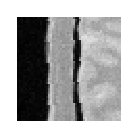
\includegraphics[width=2.5cm]{images/nn.eps}}\label{sfig:interpolation:nn}
\subfigure[]{
\includegraphics[width=2.5cm]{images/linear.eps}}\label{sfig:interpolation:lin}
\subfigure[]{
\includegraphics[width=2.5cm]{images/bs2.eps}}\label{sfig:interpolation:bs2}
\subfigure[]{
\includegraphics[width=2.5cm]{images/bs3.eps}}\label{sfig:interpolation:bs3}
\subfigure[]{
\includegraphics[width=2.5cm]{images/bs5.eps}}\label{sfig:interpolation:bs5}
\caption{Interpolation. (a) nearest neighbour, (b) linear, (c) B-spline $N=2$,
(d) B-spline $N=3$, (e) B-spline $N=5$.} \label{fig:interpolation}
\end{figure}

\section{Multi-resolution}\label{sec:comp:multiresolution}

For a good overview of multi-resolution strategies see
\citet{LesterEA99}. Part of this section is taken from the paper with
minor modifications. Two hierarchical methods are distinguished:
reduction of data complexity, and reduction of transformation
complexity.

\subsection{Data complexity}

``To reduce the number of local optima, initially the information
content within the images to be matched is reduced, so that only the
coarsest, most global structures remain. The absence of finer detail
ensures avoidance of local minima traps by virtue of their
eradication. Ideally the optimisation surface initially contains only
one maximum, in the region of the optimal global match. The
optimisation can then be improved by gradual reintroduction of
structural details at the same rate in both the images and the
concurrent updating of the registering deformation to match
corresponding re-introduced structures or features.''

``Such hierarchies of decreasing data complexity are provided by
scale spaces, where the image size is constant in all levels, or by
pyramids, where image size is also reduced in each successive level.
In the latter case, an additional advantage for pixel-based matching
schemes is that computation of optimal parameters is speeded up in
the higher level (lower resolution) images due to the reduction in
the amount of data to be processed.''

Several scale spaces or pyramids are found in the literature, amongst
others Gaussian and Laplacian pyramids, morphological scale space,
and spline and wavelet pyramids. The Gaussian pyramid is the most
common one, and we have used it all our papers.

\begin{figure}
\centering
\subfigure[]{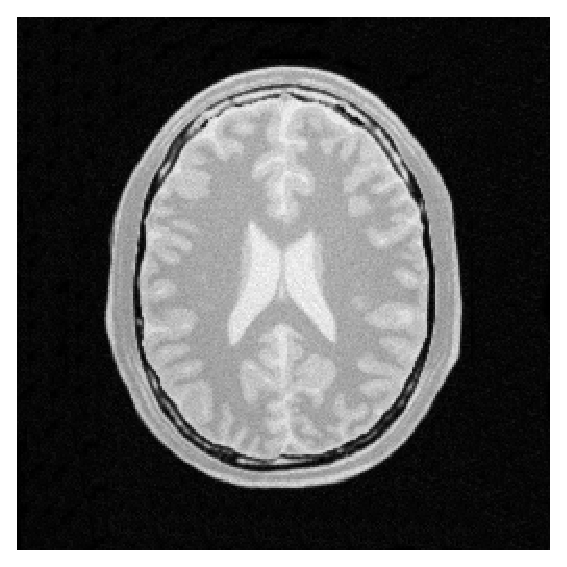
\includegraphics[width=5cm]{images/moving_pd.eps}}\label{sfig:mres:1}
\subfigure[]{
\includegraphics[width=2.5cm]{images/res2_2.eps}}\label{sfig:mres:2}
\subfigure[]{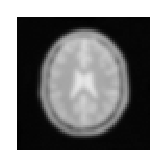
\includegraphics[width=1.25cm]{images/res1_4.eps}}\label{sfig:mres:bs3}
\caption{Multi-resolution with a Gaussian pyramid.} \label{fig:multiresolution}
\end{figure}

\subsection{Transformation complexity}

``The second hierarchical method is to increase the complexity of the
transformation within a particular algorithm.''

This is also typically used in registration, if only a rigid
registration is performed prior to nonrigid registration. Also for
the nonrigid registration part we often, but not always, apply this
technique. Registration is then started with a coarse B-spline grid,
only capable of modelling coarse deformations. In subsequent
resolutions the B-spline grid is gradually refined, thereby
introducing the capability to match smaller structures.

%%%%%%%%%%%%%%%%%%%%%%%%%%%%%%%%%%%%%%%%%%%%%%%%%%%%%%%%%%%%%%%%%%%%%%%%%%%%%%%%%%%%%%%%%%%%

\chapter{\elastix}

\section{Introduction}

The development of \elastix started half to late 2003, and was
intended to facilitate our registration research. After some initial
versions we decided to put the separate components of \elastix in
separate libraries. This resulted in major version 3.0 in November
2004. \elastix 3.0 was also the first version that was made publicly
available on the \elastix website, around the same time. The
continued development brings us today (November 2007) to version 3.7.

The website: \texttt{www.isi.uu.nl/Elastix}

CVS repository (hosted at the ISI): \texttt{/user/port/??}

History, website, where to find stuff, cvs place, where to find the
FAQ

general code layout

\section{How to use \elastix}

\section{The parameter file}

%%%%%%%%%%%%%%%%%%%%%%%%%%%%%%%%%%%%%%%%%%%%%%%%%%%%%%%%%%%%%%%%%%%%%%%%%%%%%%%%%%%%%%%%%%%%

\chapter{\transformix}

\section{Introduction}

the time \transformix takes is built up of the following parts:

1. computing the b-spline decomposition 2. computing the deformation
for each voxel 3. interpolating the input image for each voxel.

I'm not sure, but I guess step 2 is the most time-consuming task, in
case of a B-spline deformation. For a nD B-spline deformation,
computing the deformation vector at a voxel basically amounts to n
interpolations.

Step 1. is avoided by using a linear interpolator of course.

Step 3 is faster when using linear interpolation instead of cubic
interpolation. I don't know how much exactly.


What is the complexity of FinalBSplineInterpolator? And of
FinalLinearInterpolator? In required operations per voxel. Is that
described in the docs, in some papers, or on the wiki?


\section{How to use \transformix}

\section{The transform parameter file}

%%%%%%%%%%%%%%%%%%%%%%%%%%%%%%%%%%%%%%%%%%%%%%%%%%%%%%%%%%%%%%%%%%%%%%%%%%%%%%%%%%%%%%%%%%%%

\chapter{Tutorial}


\section{General advice}

\section{Important parameters}

what to tune and what not to tune

\section{Trouble shooting}

\section{Masks}

%%%%%%%%%%%%%%%%%%%%%%%%%%%%%%%%%%%%%%%%%%%%%%%%%%%%%%%%%%%%%%%%%%%%%%%%%%%%%%%%%%%%%%%%%%%%

\chapter{Developers guide}

\section{Setup of the code}

\section{Creating new modules}

%%%%%%%%%%%%%%%%%%%%%%%%%%%%%%%%%%%%%%%%%%%%%%%%%%%%%%%%%%%%%%%%%%%%%%%%%%%%%%%%%%%%%%%%%%%%

\newpage
\pagestyle{plain} \addcontentsline{toc}{chapter}{Bibliography}
\bibliographystyle{plainnat}
\bibliography{IEEEabrv,manual}

\end{document}
